% UICTEST.TEX
% This is a test file for my port of UICTHESI
% to LaTeX 2e. This is based in part on UCTHESIS.
%

\documentclass{uicthesi}




\usepackage{booktabs} % For formal tables

\usepackage{framed}
\usepackage{hyperref}
\usepackage{balance}
\usepackage[dvips]{graphics,color}

\usepackage{epsfig}
\usepackage{color}
\usepackage{subfigure}
\usepackage{multirow,tabularx}
\usepackage{placeins}
%\usepackage{miniltx}
\usepackage{mathtools}
\usepackage{graphicx}
\usepackage{epstopdf}
\usepackage{bm}

\usepackage{csquotes}
\usepackage{array}
\usepackage[yyyymmdd,hhmmss]{datetime}
\usepackage[subject={Todo}]{pdfcomment}
\usepackage[textsize=scriptsize,bordercolor=black!20]{todonotes}
\usepackage{xcolor,colortbl}
\usepackage{amssymb}% http://ctan.org/pkg/amssymb
\usepackage{pifont}% http://ctan.org/pkg/pifont
\usepackage[algo2e,titlenumbered,ruled]{algorithm2e} 
\usepackage{lipsum,environ,amsmath}
\usepackage{slashbox,booktabs,amsmath}
%\usepackage{todonotes}
\usepackage{cite}

\usepackage{xspace}

\hyphenation{PageRank Convex dictatorship Dic-ta-tor-ship}

\newcounter{Lcount}
\newcommand{\numsquishlist}{
   \begin{list}{\arabic{Lcount}. }
    { \usecounter{Lcount}
 \setlength{\itemsep}{-.1ex}      \setlength{\parsep}{0ex}
      \setlength{\topsep}{0ex}       \setlength{\partopsep}{0ex}
      \setlength{\leftmargin}{1em} \setlength{\labelwidth}{1em}
      \setlength{\labelsep}{0.1em} } }
\newcommand{\numsquishend}{\end{list}}

\newcommand{\squishlist}{
   \begin{list}{$\bullet$}
    { \setlength{\itemsep}{-.1ex}      \setlength{\parsep}{0ex}
      \setlength{\topsep}{0ex}       \setlength{\partopsep}{0ex}
      \setlength{\leftmargin}{.8em} \setlength{\labelwidth}{1em}
      \setlength{\labelsep}{0.5em} } }
\newcommand{\squishend}{\end{list}}



\makeatletter
\DeclareOldFontCommand{\rm}{\normalfont\rmfamily}{\mathrm}
\DeclareOldFontCommand{\sf}{\normalfont\sffamily}{\mathsf}
\DeclareOldFontCommand{\tt}{\normalfont\ttfamily}{\mathtt}
\DeclareOldFontCommand{\bf}{\normalfont\bfseries}{\mathbf}
\DeclareOldFontCommand{\it}{\normalfont\itshape}{\mathit}
\DeclareOldFontCommand{\sl}{\normalfont\slshape}{\@nomath\sl}
\DeclareOldFontCommand{\sc}{\normalfont\scshape}{\@nomath\sc}
\makeatother


\newcounter{problem}
\newenvironment{problem}[1][htb]
  {\renewcommand{\algorithmcfname}{Problem}% Update algorithm name
   \begin{algorithm2e}[#1]%
   \SetAlFnt{\small}
    \SetAlCapFnt{\small}
    \SetAlCapNameFnt{\small}
    \SetAlCapHSkip{0pt}
  }{\end{algorithm2e}}
  
  \newenvironment{alprocedure}[1][htb]
  {\renewcommand{\algorithmcfname}{Procedure}% Update algorithm name
   \begin{algorithm2e}[#1]%
    \SetAlFnt{\small}
\SetAlCapFnt{\small}
\SetAlCapNameFnt{\small}
\SetAlCapHSkip{0pt}
\IncMargin{-\parindent}
   
  }{\end{algorithm2e}}
  


\begin{document}

% Declarations for Front Matter

\title{Asynchronous Delegation and its Applications}
\author{George Dill}
\pdegrees{BSc (Purdue University, West Lafayette, IN) 2008}
\degree{Master of Science in Computer Science}
\committee{Prof. Jakob Eriksson, Chair and Advisor \\ Prof. Xingbo Wu  \\ Prof. William Mansky \\ }
\maketitle


% \dedication
% {\null\vfil
% {\large
% \begin{center}
% To myself,\\\vspace{12pt}
% Perry H. Disdainful,\\\vspace{12pt}
% the only person worthy of my company.
% \end{center}}
% \vfil\null}


 \acknowledgements
{The thesis has been completed... (INSERT YOUR TEXTS)\\ 

\begin{flushright}YOUR INITIAL\end{flushright}}
% \acknowledgements
% {I want to ``thank'' my committee, without whose ridiculous demands, I
% would have graduated so, so, very much faster.}

% \preface
% This preface is purely optional at UIC.

\preface


\tableofcontents
\listoftables
\listoffigures
\listofabbreviations
\begin{list}
{}
{\setlength
  {\labelwidth}{1in}
    \setlength{\leftmargin}{1.5in}
    \setlength{\labelsep}{.5in}
    \setlength{\rightmargin}{\leftmargin}}
\item[AMS\hfill] American Mathematical Society
\item[CPU\hfill] Central Processing Unit
\item[CTAN\hfill] Comprehensive \TeX\ Archive Network
\item[FIFO\hfill] First In First Out
\item[NUMA\hfill] Non Uniform Memory Access
\item[TUG\hfill] \TeX\ Users Group
\item[UIC\hfill] University of Illinois at Chicago
\item[UICTHESI\hfill] Thesis formatting system for use at UIC.
\end{list}
 
\summary
Synchronization by delegation has been shown to increase total throughput in highly parallel systems over coarse grained locking, \cite{ffwd} but the latency inherent in passing messages between cores introduces a bottleneck in overall throughput. To mitigate the effects of this bottleneck we introduce parallelism in message passing by enabling asynchronous delegation calls. 

We present two designs for asynchronous delegation, dedicated and flat. In dedicated delegation hardware threads act exclusively as a client or server as opposed to flat delegation where hardware threads share duty as both client and server. 

We compare the designs and throughput of asynchronous delegation to that of  FFWD \cite{ffwd} and Gepard \cite{gepard}, as well as to the performance of other lock-free benchmarks. 
%For a practical application, we refactor Jellyfish, \cite{jellyfish} a DNA counting program, to work with delegation and compare its performance to the stock program. 

Further, we examine the effects of hardware on the performance of asynchronous delegation and provide guidance to programmers for tuning their systems. 

\chapter{Background and Motivation}
\section{Synchronization}
Threads operating on the same memory space encounter a data race when they are simultaneously reading and modifying the same memory address. This condition results in a non-deterministic outcome of the program. 

For access to individual words, locked atomic instructions provide a guarantee that a write will be seen consistently across all threads. The guarantee is made by locking the system bus or in the processor's cache coherency policy \cite{IntelDevelopersManual}. The locked operations are slower than their standard counterparts; for example the locked compare and exchange instruction, LOCK CMPXCHG, on Intel Skylake takes 18 cycles while a CMPXCHG  instruction takes 6 \cite{agner}. 

The compare and exchange instruction can be used to implement a mutual exclusion (mutex) lock. Upon a successful write to the lock variable using LOCK CMPXCHG a thread can proceed to perform a more complicated critical section using non-atomic instructions, and then release the lock. The effect is accesses to the shared memory are serialized and threads without access to the lock end up waiting until the lock is available to do useful work. 

\section{Delegation}
\begin{figure}[ht!]
\centering
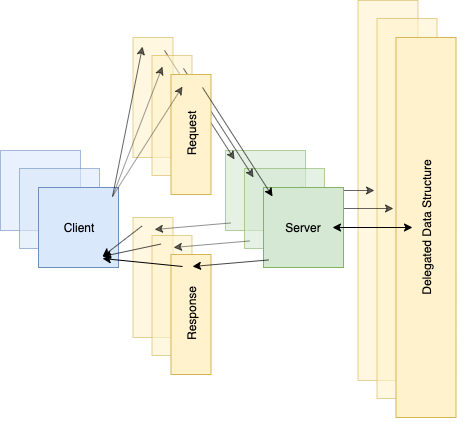
\includegraphics[width=0.9\columnwidth]{FIG/general_delegation.png}
\caption{A delegation system with 3 clients and 3 servers. The foreground client makes a request to all three servers. }
\label{fig:general_delegation}
\end{figure}
Delegation, on the other hand, provides exclusive control over a block of memory addresses to a single thread called a \textit{server}. Servers receive requests to perform an operation on their memory from other threads called \textit{clients} via a 64 Byte struct containing a function pointer, up to 6 arguments, and a status flag. Similarly responses are communicated via a 16 Byte struct containing a return value and a status flag.  

Every server-client pair has at least one dedicated request line and one dedicated response line. ~\ref{fig:general_delegation} shows a system with 3 clients and 3 servers. The client in the foreground makes a request to its allocated request line on all three servers. The server performs an operation in its delegated memory space, and writes the response to the response line allocated to that specific client. Since each request and response line has only one writer, there is no data race. 

Each delegation \textit{server} iterates through an array of requests. When a new request is encountered the server moves the variables included in the request to the appropriate registers and then calls the function pointer. The server stores the return value from the function and the flag variable into an array of responses. 

\textit{Clients} maintain an array of request pointers targeting the client's assigned request line on each server. Likewise \textit{clients} also maintain an array of pointers to the servers' responses. A client identifies a response is ready when it reads that the flag in the response is equal to the value it was set to in the request. 

An advantage of delegation is spatial locality of memory. A block of memory accessed exclusively by a delegation server is never shared with another thread. When the delegated memory block is sufficiently small, the entire working memory may fit within a server's higher levels of cache and remain resident for the duration of the program. In contrast, a system with multiple physical cores accessing the same size memory block will share cache lines, greatly reducing the likelihood of a higher level cache hit. 

From the client perspective, a drawback of delegation is the latency from request issuance to response. In ffwd, a synchronous delegation system, clients issue a request to the server's request line and then poll the respective response line until the request is returned. The time to complete a single delegated operation includes the time to write to the server, perform the function, and then receive the response. 

Gepard introduces concurrency in delegation operations while maintaining a synchronous appearance to the programmer by enabling a thread to switch to productive work through the use of fibers. Gepard clients write a delegation request to the server then make a rapid context switch to another working client fiber. After some time the client fiber will be reactivated, read its response, and then begin the cycle over again. Although the latency of a single request remains nearly constant, the overall throughput is increased by issuing parallel requests. 

Gepard shows XXpc increased throughput from ffwd on XX benchmark by issuing parallel requests. However, we see that Gepard servers are capable of handling many more requests per second than can be provided by Gepard clients. If the programmer can tolerate an asynchronous paradigm 

\chapter{Asynchronous Delegation Design}
\subsection{General}
\begin{table}\small
  \begin{description}
  \item[\bf Launch\_Servers()] Starts a server thread, allocates and initializes the request and response lines.
  \item[\bf Delegate\_Thread\_Create(f, arg)] Allocates and initializes a pending request queue for every server as thread local variable. Launches an OS thread to run function f with argument arg.   
  \item[\bf Delegate\_Async(s, cb, f, args...)]  Generates a delegation request to server s with function f and arguments args. Calls cb with the return value from f.
  \item[\bf Delegate\_Async\_Barrier()] Places requests from a delegated thread's queue and polls server responses until all requests have been served. 
\end{description}
\caption{Excerpt of the asynchronous delegation API. }
\label{t:api}
\end{table}
In \textit{Gepard} and \textit{FFWD} the client application blocks after issuing a request until a response is received from the server. \textit{Gepard} hides the waiting time for the return value by switching fibers during this waiting period. However if we can tolerate an asynchronous programming model we can expose greater concurrency without the overhead of switching user space fibers. 

The difference is evident in the change to the API. While \textit{Gepard} and \textit{FFWD} make a call to \textbf{delegate(s, retval, f, args)} and require a return value, asynchronous delegation makes a call to \textbf{Delegate\_Async(s, cb, f, args)} where cb is a callback function with the return value as a parameter. For most invocations a call to \textbf{Delegate\_Async(s, cb, f, args)} is non-blocking. 
The entire API of asynchronous delegation is shown in ~\ref{t:api}. 

The strategy for issuing requests to the delegation servers varies in the asynchronous designs detailed below. 


\section{Dedicated Delegation}
\begin{figure}[ht!]
\centering
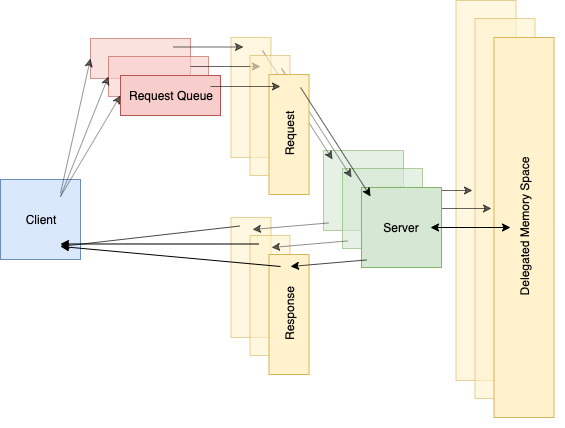
\includegraphics[width=0.9\columnwidth]{FIG/dedicated_async.png}
\caption{A delegation system with 1 client and 3 servers. The foreground client makes a request to all three servers. Requests are written to a pending request buffer which is periodically flushed out to the request line. }
\label{fig:flat_delegation}
\end{figure}

To use dedicated delegation the user must first initialize a number of delegation servers using \textbf{Launch\_Servers}. Running on separate OS threads, the servers begin sequentially polling their request lines. The user then launches OS threads with the application code by calling \textbf{Delegate\_Thread\_Create}. When a thread is started with \textbf{Delegate\_Thread\_Create} an empty queue of pending requests for each running server is allocated on the client's NUMA node. 

Within the application code the programmer uses \textbf{Delegate\_Async} to enqueue a pending request. When any of the pending request queues is filled, the client works through its entire list of responses. When a response is ready, the client invokes the callback with the corresponding return value, and then writes a new request to the corresponding request line from the pending request queue. 

At any time the user can call \textbf{Delegate\_Async\_Barrier} to ensure that all outstanding requests are served before moving on.  \textbf{Delegate\_Async\_Barrier} is always called upon return of the application code. 

\section{Flat Delegation}
\begin{figure}[ht!]
\centering
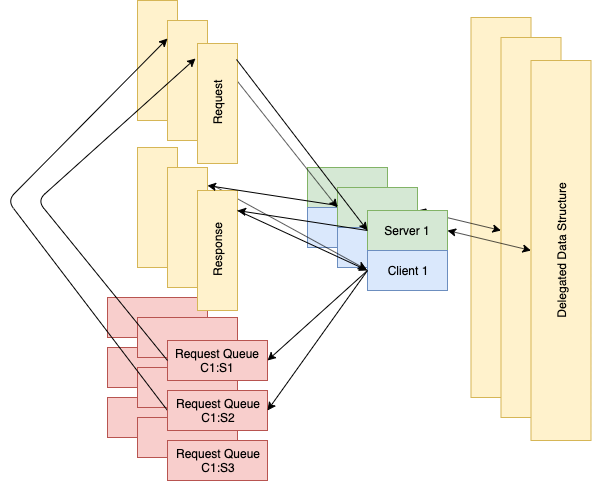
\includegraphics[width=0.9\columnwidth]{FIG/flat_async.png}
\caption{A flat delegation system with 3 client-server threads. The foreground client makes a request to itself. The background client makes a request to the foreground server. }
\label{fig:flat_delegation}
\end{figure}

Flat delegation runs clients and servers on the same thread. There is no call to \textbf{Launch\_Servers}, instead servers are initialized upon the call to \textbf{Delegate\_Thread\_Create}. ~\ref{fig:flat_delegation} illustrates how the same hardware thread works as both client and server. Each thread must make progress on its client's work while balancing availability to serve the requests which it has been assigned. 

Like Dedicated Delegation, the programmer makes calls to \textbf{Delegate\_Async}. However, the number of client-server pairs in flat delegation is 
\begin{displaymath}
(number of threads)^2 
\end{displaymath}
compared to 
\begin{displaymath}
(number of clients) * (number of servers)
\end{displaymath} 
for dedicated. Maintaining the pending request queues for each client-server pair easily exhausts the L1 cache. Instead, requests are written directly to the server's request line. 

The direct request line write is handled as follows: The client keeps track of the most recently used request line on a server. Upon a \textbf{Delegate\_Async} call, the next response line is handled if available. After handling the response, if the request line is free the request is written out. An unavailable request line implies that this client is waiting on another server. The thread remains productive by serving all of its request lines and then returning to the client. The client will continue invoking the server until its desired request line becomes available. 

Like dedicated delegation, \textbf{Delegate\_Async\_Barrier} is invoked to ensure that all outstanding requests and responses are handled before joining. 

\section{Ordering Guarantees}
\begin{figure}[ht!]
\centering
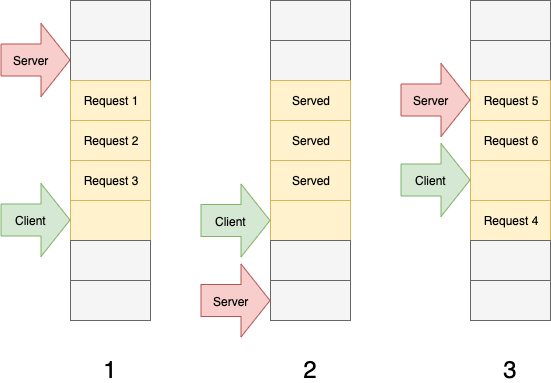
\includegraphics[width=0.9\columnwidth]{FIG/multiple_rl_race.png}
\caption{The server may execute requests out of order when multiple requests lines are used by one client. (1.) The client issues 3 requests before the server reaches its section of the request line array. (2.) The server handles all requests in this clients section before the client writes a fourth request. (3.) The client writes its next request into the next available line, after request 4 is written the next line is the first one. The requests are now executed out of order.}
\label{fig:mulitple_rl_race}
\end{figure}
Beyond the concurrency we can achieve by writing to multiple servers at once, we can also pass multiple requests to the same server simultaneously. To do this we increase the number of request lines available to a client on each server. 

Servers handle requests by iterating through all of their request lines and performing those requests with the appropriate flag. However, when there are multiple request lines per server-client pair we cannot guarantee that the requests will be performed in the order they are sent. Consider the case shown in ~\ref{fig:multiple_rl_race}.  A client writes a request to all but one of its request lines before the server handles the entire batch. Afterward the client writes requests to its last request line and then begins writing new requests to its first request line. Since the server handles requests in the order of the request line array, newer requests are handled before the oldest request in the last position. 

For an application with non-commutative properties a single request line preserves the ordering of requests made by a client to a specific server. Experimental results are shown with both 1 and 16 request lines per client-server pair to show the difference in throughput while maintaining ordering. 

%An asynchronous delegation client initializes a FIFO queue for each available server.  The queue is implemented as a fixed size circular array so that memory can be allocated once upon the creation of the client thread. When an asynchronous delegation request is generated by the application, the \textbf{Delegate_Async} call attempts to enqueue the request. If the queue is not full, \textbf{Delegate_Async} returns and the client program can resume execution. When the queue is full, \textbf{Delegate_Async} cycles through each of its dedicated request and response lines. When a response line indicates a matching response to a request, the call back function is run on the return value and a new request is written if available. 

\chapter{Experimental Evaluation}
The following results shown are from a 28 core, 56 thread Intel Skylake machine with 97 GB of RAM, 32kB of L1 cache, 1,024KB of L2 cache, and 19,712kB L3 cache shared among the 14 physical cores on each socket. 

For locking, atomic operations, and flat delegation we use the number of threads available on the machine (56) unless stated otherwise. For trials with the dedicated organization we list the number of servers. The balance of remaining threads are clients.  The client and server ratio is selected by the best results with 1 variable per server. 

Like \textit{Gepard}, asynchronous delegation threads are assigned to cores in a round-robin fashion. In the dedicated case all server threads are launched before any client threads. Memory for delegated data structures is allocated on the NUMA node corresponding to the server which it is assigned. 

Results shown are the weighted arithmetic mean performance over 10 runs of three seconds or greater. 

\section{Fetch and Add Performance}
\begin{figure}[ht!]
\centering
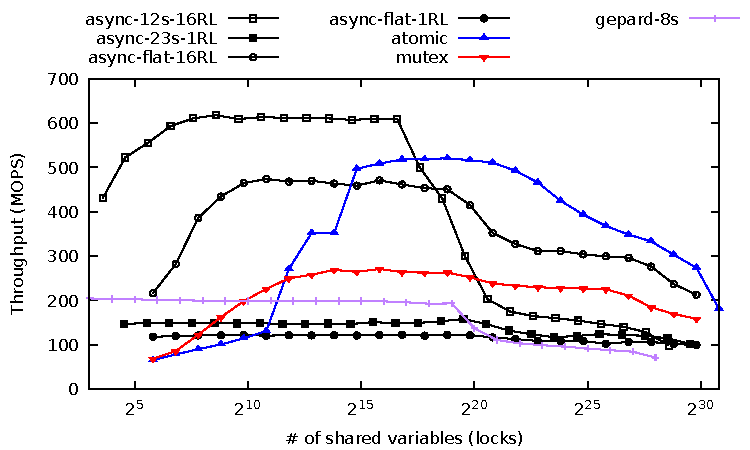
\includegraphics[width=0.9\columnwidth]{FIG/fetch_and_add_thput.pdf}
\caption{Throughput in MOPS by number of 64Byte variables. Higher is better. }
\label{fig:fetch_and_add_thput}
\end{figure}

The experiment shown in ~\ref{fig:fetch_and_add_thput} selects a variable at random and then increments it using the synchronization type shown. Each variable is 64 Bytes and 64 Byte aligned. For the locking case the lock takes the place of padding in the variable struct. There is one lock per variable. 

Delegation approaches excel for smaller numbers of shared variables. Notice dedicated delegation achieves over 600 MOPS for shared variable counts up to the size of the server cache. Flat delegation achieves consistent performance, topping out near 500 MOPS. The reason for this even performance at low levels of shared variables is a lack of contention.

A variable is contended if multiple threads are trying to access it simultaneously. Neglecting interleaving due to time, the chance that at least one pair of threads in the system are contending for a variable is plotted in ~\ref{contention} and described as follows. : 
\begin{displaymath}
contention = 1 - {{ variables \choose threads }  \over  variables^{threads}}
\end{displaymath}
\begin{figure}[ht!]
\centering
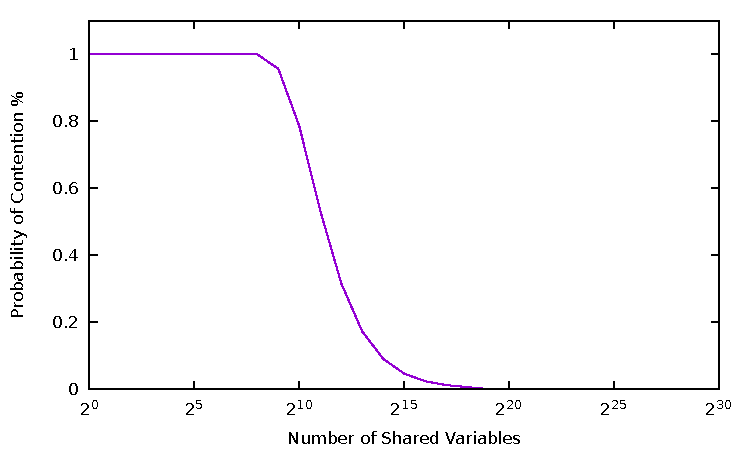
\includegraphics[width=0.9\columnwidth]{FIG/contention.pdf}
\caption{Probability that at least one pair of threads is contending for a variable}
\label{fig:contention}
\end{figure}

Delegation servers do not contend for variable access by design. In contrast the fine grained lock and the atomic fetch and add have up to 56 threads accessing a single memory location. ~\ref{fig:fetch_and_add_thput} shows the atomic fetch and add and the fine grained mutex reach peak performance as the probability of contention reaches 0 ~\ref{fig:contention}. For quantities of shared variables smaller than the size of a single processors cache contention should be evident in L3 cache hits. More L3 cache hits indicate more contention because uncontended variables should remain in a processors exclusive L1 or L2 cache. ~\ref{fig:contention} shows delegation approaches with fewer L3 cache hits per operation compared to the atomic fetch and add and the fine grained mutex lock. 

On the opposite end of the scale delegation performance degrades as the number of shared variables increases. 
\begin{displaymath}
{P(In Cache)_{delegation}} = {{L2BytesAvailable} \over { size of shared variables / number of servers}}
\end{displaymath}
As the probability that a variable is in cache approaches zero the time to access DRAM dominates the performance of the delegation server. Flat delegation offers an improvement to other delegation designs in this region because it maintains the same number of threads making memory accesses while ensuring that all DRAM access are local to the thread's NUMA node. 

\section{Design Parameters for Dedicated Delegation}

Figure: max throughput by client-server combination for all cores case
	Discussion production rate of clients, consumption rate of clients
Figure: Throughput by number of request lines
Figure: Throughput by size of ring buffer, no ring buffer
	Server and Client hit rate

\section{Design Parameters for Flat Delegation}

Figure: Throughput by schedule type
	Server and client hit rate

\chapter{Conclusions}
Flat provides and easier API, no tuning. 
%Validate - does it extend the performance for larger data structures?
Dedicated allows the user to adjust the producer / consumer rates
Applications are programs with smallish data structures with operations more complicated than compare and swap. 


%\chapter{Some other stuff I wrote but probably shouldn't be included}
%\section{Hardware}
%Under consideration is our highly parallel machine consisting of multiple processing units, or cores, sharing resources on a single silicon processor. Cores execute threads, or sequences of machine instructions. X86 machines often support the simultaneous execution of two threads at the same time. In this hyperthreaded scenario a core's resources are shared between the threads in execution. 
%
%Processors are installed in sockets on the machine's motherboard. The processors on separate sockets communicate with each other through a bus. On a machine supporting Non Uniform Memory Access (NUMA) each socket is also a NUMA Node, with direct access to a portion of main memory (DRAM). Cores on a socket will experience greater latency accessing memory addresses on a remote NUMA node than memory addresses resident on their local NUMA node because of the time required for the data to travel across the bus. 
%
%Access to main memory is a bottleneck for modern processors, which can perform an operation in as little as 1 cycle but write to memory in the order of LOOK THIS UP. To close this latency gap processors and cores have levels of cache, small amounts of high speed memory located closer to the processing unit. Cache is typically allocated in three levels, with levels 1 and 2 dedicated to a single core, while level 3 is shared among all cores on a processor. The latency of access to levels 1, 2, and 3 is around 5, 15, 60 cycles respectively. 
%
%The cache optimization works by making a working copy of the data at a memory address and moving it into the lower latency memory closer to the core. The core can manipulate this memory locally and write it out to main memory when it is complete. When access to a memory address is predictable or frequent, data at memory addresses can be moved ahead of time, or prefetched, to the cache, and the core can benefit from the lower latency of the cache memory.   
%
%Although memory is byte addressed, the cache system manages information in 64 byte segments called cache lines. Caches are typically n-way set associative. A set can hold up to n cache lines which share a common portion of their memory address. 
%
%For example, a 32kB 8-way set associative cache has 512 cache lines split into 64 sets. Each set accepts memory addresses with bits 6-11 of the memory address in common. 
%
%When a cache is full, the least recently used cache line is evicted to a lower level cache or main memory in favor of a newer cache line. 
%
%When multiple cores access memory in the same cache line the copies resident in each core's cache may become inconsistent. Cores can snoop on another core's cache line status. If a core detects that a cache line has been modified on another core, the snooping core signals the modifying core which then forwards the modified cache line, causing an increase in access time\cite{IntelDevelopersManual}. In a concurrent program multiple cores may be writing to separate addresses resident in the same cache line. The cache line is shared between cores although the memory addresses are not. This false sharing of the memory addresses increases access latency for all cores operating on the cache line. 
%
%\section{Schemes for Shared Memory Access}
%Of course concurrent programs not only false share cache lines, they perform operations on the same memory addresses as well. Without careful synchronization by the programmer multiple cores can read and modify a memory address concurrently producing a non-deterministic result. Some of the methods for preventing this data race are described below. 
%% Locking
%Mutual Exclusion (Mutex) locks synchronize memory access through a variable that a thread must claim before moving forward with its data altering, or critical, section. When a competing thread views the lock as occupied it will wait to execute its critical section until it gets exclusive control of the lock. 
%
%There are several ways of implementing the MUTEX lock. // expand upon this.  
%
%Regardless of the implementation, synchronization schemes using locks suffer bottlenecks due to sharing the lock variable across multiple processors or sockets. In fine grained locking schemes these lock variables may take up a significant portion of memory (validate this). Additionally, memory modified in the critical section may reside in another cache, local DRAM, or another NUMA node's DRAM. 
%% Atomic Operations
%Atomic operations are those operations where 
%% Transactional Memory
%
%
%
%\chapter{Rates and System Performance}
%% Quantifying the client - server relationship
%% 



This is how we cite a paper \cite{Farine20162243}.

Below is the example of algorithm block.


\IncMargin{1em}
\begin{alprocedure}[!htp]
\caption{FindFactionsAndInitiators}
\SetKwInOut{Input}{input}\SetKwInOut{Output}{output}
\Input{An adjacency matrix $E^*$ of dynamic network}
\Output{ A time series of faction sets $\mathcal{F}^*$, and a time series of initiator sets $\mathcal{L}^*$ }
\BlankLine
\For{$i\leftarrow 1$ \KwTo $t^*$}{
\textcolor{cyan}{\tcc*[h]{Get a matrix at time $t=i$} }

$E \leftarrow E^*_{ t = i}$ \; 
\textcolor{cyan}{\tcc*[h]{FindInitiators($E $) returns all nodes which have zero outgoing degree}}

$\mathcal{L} \leftarrow$FindInitiators($E $) \;
$\mathcal{F} = \emptyset$ \;
\For{$l \in \mathcal{L}$}{
\textcolor{cyan}{\tcc*[h]{FindReachNodeFrom($E,l$) returns all nodes which have any directed path to $l$}}

$F_l\leftarrow$FindReachNodeFrom($E,l$) \;
$\mathcal{F} = \mathcal{F} \cup \{F_l\}$
}
$\mathcal{F}^*_{t=i} = \mathcal{F}  $ and $\mathcal{L}^*_{t=i} = \mathcal{L}  $
}
\label{algo:FindFactionsAndInitiators}
\end{alprocedure}\DecMargin{1em}


The example of table is below.

\begin{table}[!htp]
\tiny
\centering
\caption{Table Caption1}
\label{table:htestdes}
\begin{tabular}{l|l|l|}
\cline{2-3}
                                                                                                                     & \cellcolor[HTML]{EFEFEF}\textbf{Method}                                    & \cellcolor[HTML]{EFEFEF}\textbf{Null hypothesis $H_0$}                                                                                          \\ \hline
\multicolumn{1}{|l|}{}                                                                                               & $t$-test                                                                      & \begin{tabular}[c]{@{}l@{}}A sample has a normal distribution \\ with zero mean and unknown variance.\end{tabular}                              \\ \cline{2-3} 
\multicolumn{1}{|l|}{}                                                                                               & \cellcolor[HTML]{EFEFEF}Sign test                                          & \cellcolor[HTML]{EFEFEF}A sample has a distribution with zero median.                                                                           \\ \cline{2-3} 
\multicolumn{1}{|l|}{\multirow{-3}{*}{\textbf{\begin{tabular}[c]{@{}l@{}}Zero \\ mean/median \\ test\end{tabular}}}} & Wilcoxon signed rank test                                                  & A sample has a symmetric distribution around zero median.                                                                                       \\ \hline
\multicolumn{1}{|l|}{}                                                                                               & \cellcolor[HTML]{EFEFEF}Kolmogorov-Smirnov test (KS test)                           & \cellcolor[HTML]{EFEFEF}A sample comes from a normal distribution.                                                                              \\ \cline{2-3} 
\multicolumn{1}{|l|}{}                                                                                               & \begin{tabular}[c]{@{}l@{}}Chi-square \\ goodness-of-fit test\end{tabular} & \begin{tabular}[c]{@{}l@{}}A sample comes from a normal distribution \\ with a mean and variance estimated from a sample itself.\end{tabular}   \\ \cline{2-3} 
\multicolumn{1}{|l|}{}                                                                                               & \cellcolor[HTML]{EFEFEF}Jarque-Bera test                                   & \cellcolor[HTML]{EFEFEF}\begin{tabular}[c]{@{}l@{}}A sample comes from a normal distribution \\ with an unknown mean and variance.\end{tabular} \\ \cline{2-3} 
\multicolumn{1}{|l|}{\multirow{-4}{*}{\textbf{\begin{tabular}[c]{@{}l@{}}Normality \\ test\end{tabular}}}}           & Anderson-Darling test                                                      & A sample comes from a normal distribution.                                                                                                      \\ \hline
\end{tabular}
\end{table}



\section{Support of leading faction}

\begin{figure}[ht!]
\centering
\includegraphics[width=0.9\columnwidth]{FIG/CoorEventSup}
\caption{An example of image in thesis }
\label{fig:CoorEventSup}
\end{figure}


 \appendices
 \newpage
 \appendix

 \chapter{Some Ancillary Stuff}

 Ancillary material should be put in appendices.

 \chapter{Some More Ancillary Stuff}

% Here is yet another appendix! Wahoo!

%\nocite{*}
\bibformb
\bibliography{BibFile}
\newpage
% \vita
% This is where the vita goes.  Its organization is left as an exercise.
\clearpage
    \pagestyle{pageontop}
   \thispagestyle{pageonbottom}
   %\vspace*{3in}
   \begin{large}
   \begin{center}
   {\bfseries VITA}
   \end{center}
   \end{large}
\begin{tabular}{p{2.8cm}p{10.5cm}}
NAME: & NAME LASTNAME  \\ 
    &\\
EDUCATION:  &Ph.D., Computer Science, University of Illinois at Chicago, Chicago, Illinois, 2018. \\  
            &\\
            &M.Eng., Computer Engineering, University of Illinois at Chicago, Chicago, Illinois, 20xx.\\
            &\\
            &B.Eng., Computer Engineering, University of Illinois at Chicago, Chicago, Illinois, 20xx.  \\
            &\\
ACADEMIC EXPERIENCE:  &Research Assistant, Computational Population Biology Lab, Department of Computer Science, University of Illinois at Chicago, xxxx - 2018. \\
            &\\
            &Teaching Assistant, Department of Computer Science, University of Illinois at Chicago: \\
            &\squishlist            
            \item Computer Algorithm I, Spring xxxx and  Fall xxxx.    
            \item Secure Computer Systems, Fall xxxx 
            \squishend \\
            

 \end{tabular}

\end{document}
